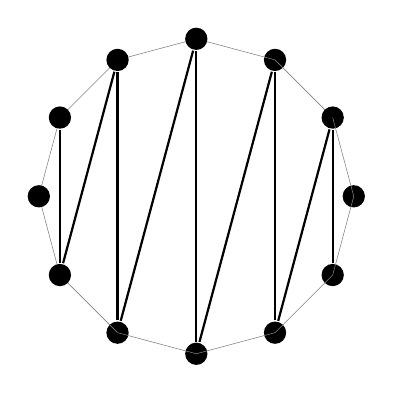
\begin{tikzpicture}[thick,inner sep=0.1cm]
	\foreach [count=\n] \t in {30,60,...,360}{
		\node [fill,circle] at (90-\t:2) (node \n) {};
		\draw [help lines] (\t:2) -- (\t+30:2);
	}
	
	\draw (node 8) to (node 10);
	\draw (node 8) to (node 11);
	
	\draw (node 7) to (node 11);
	\draw (node 7) to (node 12);
	
	\draw (node 6) to (node 12);
	\draw (node 6) to (node 1);
	
	\draw (node 5) to (node 1);
	\draw (node 5) to (node 2);
	
	\draw (node 4) to (node 2);
	
\end{tikzpicture}

